\documentclass[a4paper,11pt]{report}
\setlength{\parskip}{\medskipamount}
\setlength{\parindent}{0pt}
\usepackage{graphicx}

\begin{document}

What problem we are trying to solve?

most of the time, doing calculations on large systems doesn't need, in principle,
the calculation on the whole molecule. Usually, if we want to perform a CI
calculation on a large polyene chain, for example, we need to compute a
large seward over the whole chain, then do a delocalized CAS (2n/2n).
With localization, we saw that the 2n/2n evaluation can be, in principle,
substituted with a simple 2/2 evaluation. Then, we can freeze the orbitals,
and finally we could remove atoms from the seward treatment.

To do a CI evaluation, we need the monoelectronic integrals (TraInt) and the
bielectronic integrals. Given the evaluation of the bielectronic integrals
is a quite heavy task, if we can reduce this step our calculation efforts
will be greatly reduced.

This molecule is a long polyene chain with a C=O. Our objective is to
describe the molecule suppressing atoms that are far from the chromophore.

For the current moment we do two calculations. a big calculation and a small
calculation.

The big calculation is done over the molecule as a whole. We run a seward,
an scf, and then we localize orbitals.
The procedure is a standard localization procedure
(schmudorb,proj\_scf,schmudort) with no noscf optimization. Please note that
in this case (tridequenal) we freeze all the 1s core, and mark as active
the n and pi*.

Then we feed the localized orbitals into troncat. Its input file is here given

\begin{verbatim}
&TRONCAT prefix='tridequenal.'
 nprint_hieror=-1,
 keepl='O1','C1','C2','C3','C4','C5',
 'H1','H2','H3','H4','H5',
 eliml='C5C6'
 'H10','H11','H12','H13',
 'C10','C11','C12','C13'
 keep='C1 ','C2 ','C3 ','C4 ','C5 ','C6 ','O1',
 'H1 ','H2 ','H3 ','H4 ','H5 ','H6 ',
 'C7','H7',
 'C8','H8',
 elim='H10','H11','H12','H13',
 'C10','C11','C12','C13'    /
\end{verbatim}

there are some keywords that need an explanation:
keep is a keyword that describes the atoms that must express our orbitals.
if the algorithm for the selection with the label was "single-shot" there
were no need of elim keyword. This keyword is given since the pattern
matching is a glob-like, so keep='C1' match also C10, C11, C12 and so on, so
we need to explicitly exclude these atoms.
keepl and eliml are the same, but we need to specify the localized bonds
that we need to keep. The orbitals that we mark as eliminated using keepl
and eliml are marked as G (GELEE, frozen). So pay attention to the fact that
there are two levels of frozing: the one at the schmud, where we froze the
core, and the one at this level, where we froze everything but the small
piece at the crossing between 2 and A (see diagram)

The procedure is like this: after the run of troncat, we obtain various
output files: TRONCORBP, TRONCORBG, hiering and hierinp.
The aim of this procedure is to obtain an orbital matrix in this form (on
atomic basis)

\begin{verbatim}
before troncat

                 1  |   2   |  3
              +--------------------+
              |                    |
A) atoms kept |                    |
in both calcs |                    |
              |                    |
              |                    |
        ----- |                    |
              |                    |
B) atoms      |                    |
eliminated    |                    |
in the small  |                    |
calculation   |                    |
              +--------------------+
\end{verbatim}

\begin{figure}[ht]
\begin{verbatim}
after troncat

                 1  |   2   |  3
              +-----+---------+----+
              |     |       |d|    |
atom kept in  |     |submat |u|    |
both calcs    |     |       |m|    |
              |     |       |m|    |
              |     |       |y|    |
        ----- |     +-------+-+    |
              |     |       |      |
atoms         |     |       |      |
eliminated    |     |   0   |      |
in the small  |     |       |      |
calculation   |     |       |      |
              +-----+-------+------+
\end{verbatim}
\end{figure}

Troncat then produces TRONCORBP that contains the submat only, TRONCORBG
that contains the whole, big matrix.
Now, the orbitals in submat are no longer orthogonals. So a procedure for
reorhogonalization is needed, both for the small molecule and the big
molecule. troncorb prepares for us the input files for the subsequent
hierarchical orthonormalization.

please note that there's a point of warning: the submat is not squared, but
motra need it to be square to do the transformation. this is not a problem.
we include a little dummy piece from the virtual zone to obtain a square
matrix, and we feed the whole little matrix to motra, to transform the
integrals from atomic basis to molecular basis against the small matrix.
These orbitals are marked as G\_BID (BIDon = nonsense)

Our target is: obtain the OneInt file from the big calculation, obtain the
OrdInt (two electron integrals) from the little calculation, combine them to
start with a molcost+casdi calculation (for example, doing CAS+S or
something more interesting).

(Problem: orbitals are never optimized from a level more deeper than
SCF+localization. every subsequent calculation uses these orbitals in a CI.
it could be possible to utilize noscf to obtain a CASSCF quality orbitals,
but needs some coding. In the current implementation, orbitals are of scf
quality, except for the cutoff-reorthogonalization procedure that could
worsen this quality, the more higher are the coefficient in the cutoff zone,
the higher the quality will degrade)

in our first example of the usage of troncorb, given the molecule

\begin{verbatim}
               .        .  
       H2   H4 . H6   H8.  H10  H12
       |    |  . |    | .  |    |   
  H1   C2   C4 . C6   C8.  C10  C12  H132
   \  / \\ / \\./ \\ / \\ / \\ / \\ /
    C1   C3   C5   C7   .C9   C11  C13
    ||   |    |.   |    . |    |    |
    O1   H3   H5   H7   .H9   H11  H131
               .        .
normally   <---.<--+--->.----> removed from the orbitals (keep/elim)
kept (orb.         |
and atoms)         `---- kept as orbitals, but frozen (G)
\end{verbatim}           

we should evaluate the difference in the n->pi* excitation energy moving
both barriers.

The output for troncat reports at first the kept and elimined atomic orbitals.
Then it presents the overlap between the new orbitals (with all zeros on the
eliminated coefficients) and the old ones, and also the norm. Please note
that an increase of the norm is possible, since we are working in a basis
set that is not orthogonal. a picture will be self explaining

\begin{center}
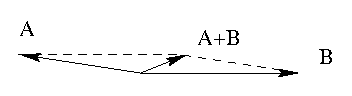
\includegraphics{vectors.eps}
\end{center}

as we can see in the output from troncorb, the orbitals starting from C1C2 are clean
(zero values) in C9 and subsequents. Note also that lines with all zeroes
are removed from the output and there's no order, so it's not impossible to
see all zeroes, then values, then zeroes (take the example of H8):

\begin{verbatim}
 111 C13 2pz    0.0000  0.0000  0.0000  0.0000  0.0000  0.0000  0.0003
-0.0009  0.0013 -0.0029
 112 C13 2pz    0.0000  0.0000  0.0000  0.0000  0.0000  0.0000 -0.0001
-0.0001  0.0005 -0.0004
 113 H8  1s    -0.0006 -0.0862 -0.0512 -0.1060 -0.1601 -0.2420 -0.0422
0.0404 -0.0564 -0.0670
 114 H8  1s    -0.0006 -0.0733 -0.0467 -0.0853 -0.1066 -0.1890  0.0021
-0.0004 -0.0013 -0.0005
 115 H9  1s     0.0000  0.0000  0.0000  0.0000  0.0000  0.0000 -0.0101
0.0507 -0.0374  0.0667
 116 H9  1s     0.0000  0.0000  0.0000  0.0000  0.0000  0.0000  0.0004
-0.0028 -0.0012  0.0005
\end{verbatim}

H8 is not cut out, so is good. This "strangeness" is only for a matter
of numerical ordering.

This procedure produces TRONCORBP and TRONCORBG that are simple INPORB type
files, and TRONCP\_MONO, monoelectronic integrals on the molecular basis set 

They are fed, in turn, into the hierarchical orthogonalization procedure:

cp TRONCORBG INPORB
cp tridequenal.Mono MONO
/work0/borini/lavoro/programs/cost-loc/bin/hieror < hiering > hieroutg
cp ORTORB ORTORBG

cp TRONCORBP INPORB
cp TRONCP\_MONO MONO
/work0/borini/lavoro/programs/cost-loc/bin/hieror < hierinp > hieroutp
cp ORTORB ORTORBP
exit

To obtain orbitals for the large and small system. Now we can produce
one electron integrals from the large systems, with motra using the options
frozen and delete to explicity exclude the orbitals, and then we need to
calculate the two electron integrals over the reduced seward system, feed
them into motra with the ORTORBP file and obtain OrdInt.

in this case, we need to delete 34 orbitals of the first simmetry and 6 of
the second simmetry (they are the last orbitals for each symmetry, and
marked as BID) for the small system, and mark

Frozen
 31 4
Delete
 50 12

for the large calculation (with the OneOnly keyword, and using the ORTORBG as orbital
fine) thus explicitly exclude the orbitals and regain the small matrix we
are interested to.

Finally, we get everything we need.



\end{document}
